\FloatBarrier
\subsection{Choose and explain the error-correcting code}
\label{sec:r32}
I select the taught systematic Hamming(7,4): length 7, four information
bits, rate $4/7 $, $ d_{\min}=3 $ and guaranteed correction $ t=1 $ \citep{hamming1950codes}.
With row messages, encoding is $\boldsymbol c=\boldsymbol mG\pmod2 $;
the receiver computes $\boldsymbol s=\boldsymbol rH^T\pmod2 $, matches
the actual $ H $ column, flips that position and extracts the four systematic
bits. The reference uses integer matrix multiplication followed by modulo two.
The exact $ G,H $, distance proof and worked examples are in
Appendix~\ref{app:ecc}. Its columns are 110, 101, 011, 111, 100, 010, 001;
a syndrome integer is not a direct bit index. This code is not SECDED:
multiple errors can be miscorrected, and a zero final syndrome does not
prove recovery of the transmitted message.

\paragraph{Alternatives, error profile and declared selection.}
The alternatives are the implemented Hamming(15,11), also $ d_{\min}=3,t=1 $;
majority-decoded repetition(5,1), $ d_{\min}=5,t=2 $; and uncoded(1,1).
The code constructions and exact decoder expectations are derived in
Appendix~\ref{app:ecc}. A higher Hamming rate does not increase correction
capability. Actual iid BSC flips produce binomial block multiplicities,
not an artificial one-flip restriction (Figure~\ref{fig:r32-profile}).
For the verified decoders, low-$ p $ BER begins at $9p^2 $ for (7,4),
versus $21p^2 $ for (15,11).

\begin{figure}[htbp]
 \centering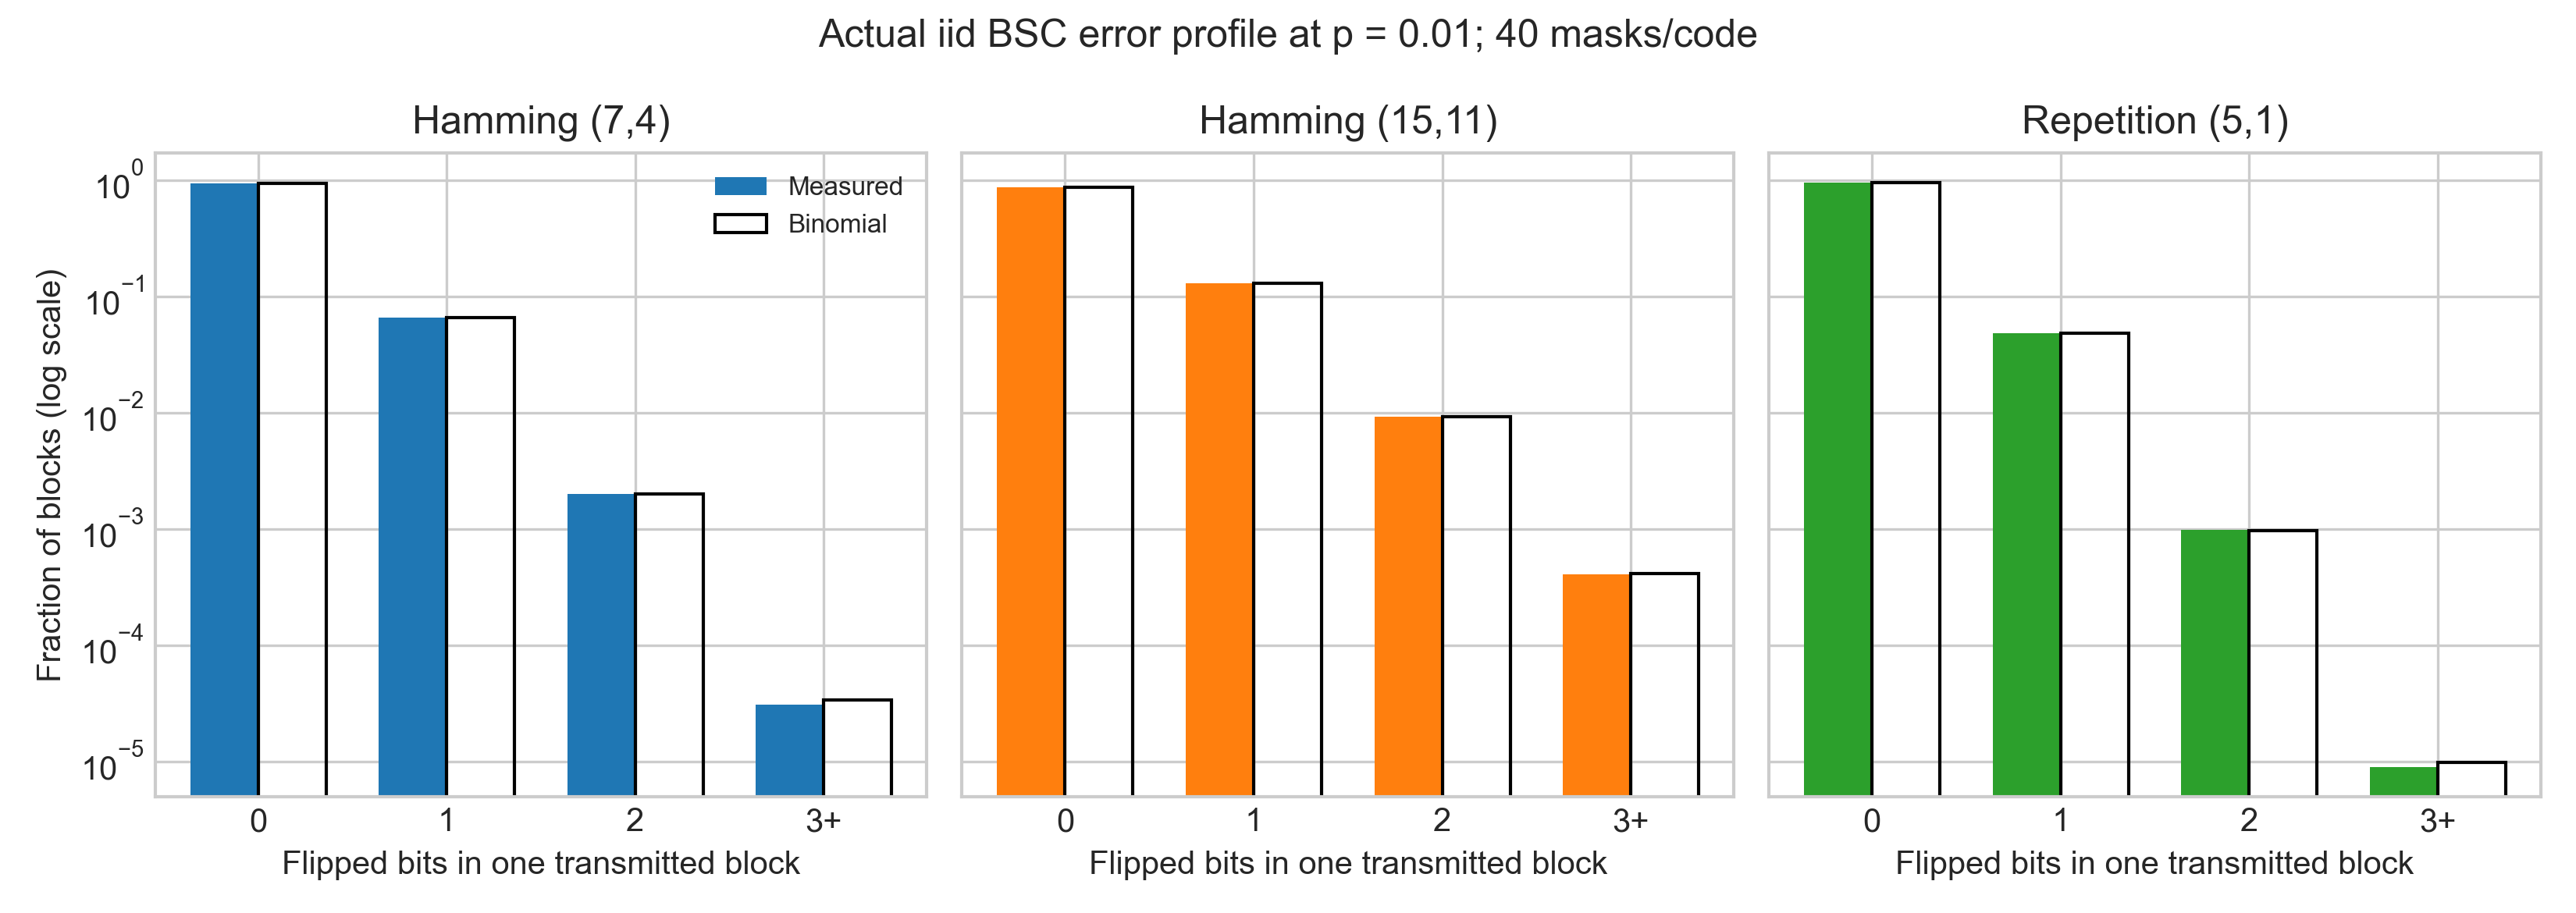
\includegraphics[width=.86\linewidth]{images/r32_block_profile.png}
 \caption{Actual BSC multiplicities versus the binomial model. Both Hamming codes correct one error; repetition corrects two at fivefold traffic cost.}
 \label{fig:r32-profile}
\end{figure}

The pilot reuses five R3.1 anchor-SNR inputs, with eight independent
masks per positive $ p $/code and one identity control per bank/code:
1140 cases, 1120 positive-$ p $ masks. The prespecified probabilities are
$0,10^{-4},0.001,0.003,0.01,0.03,0.1,0.3 $.
Five input banks are the independent units for selection; 40 masks are not
40 independent Gaussian inputs. Before BSC generation I fix expansion
$ M_t/M_b\le2 $ and equal selection weights over
$\mathcal P=\{0.001,0.003,0.01,0.03\}$:
\begin{equation}
 J_{c,g}=\frac14\sum_{p\in\mathcal P}
  \frac{\overline D_{c,p,g}}{\overline D_{\mathrm{uncoded},p,g}},
 \qquad J_c=\frac15\sum_{g=0}^4J_{c,g}.
 \label{eq:r32-score}
\end{equation}
Here $\overline D_{c,p,g}$ averages the eight full-grid MSEs in one bank.
The normalisation prevents high-$ p $ absolute loss alone determining the
score. Choose the eligible ECC with smallest $ J_c<1 $.

\begin{table}[htbp]
 \centering\small
 \caption{Defined alternatives and phase-0 selection score. Feasibility uses the declared twofold expansion budget, not the later rate cap.}
 \label{tab:r32-selection}
 \begin{tabular}{lrrrrrrr}
\toprule
Code & $n$ & $k$ & $d_{\min}$ & $t$ & Expansion & kbit/s & $J$ \\
\midrule
Uncoded & 1 & 1 & 1 & 0 & 1.00000 & 224 & 1.00000 \\
Hamming (7,4) & 7 & 4 & 3 & 1 & 1.75000 & 392 & 0.08344 \\
Hamming (15,11) & 15 & 11 & 3 & 1 & 1.36366 & 305.46 & 0.19204 \\
Repetition (5,1) & 5 & 1 & 5 & 2 & 5.00000 & 1120 & 0.01920 \\
\bottomrule
\end{tabular}

 
 
\end{table}

Hamming(7,4) has $ J=\ECCScore $, approximate pointwise 95 \% interval
$[\ECCScoreLow,\ECCScoreHigh]$, against 0.19204 for (15,11).
The paired difference is $-0.10860 $, interval $[-0.11311,-0.10410]$.
Repetition improves further ($ J=0.01920 $) but needs fivefold expansion.
A 1.5/2/5-fold budget would instead select (15,11)/(7,4)/repetition;
the twofold budget is a project resource preference, not a physical limit.

\paragraph{Framing, waveform meaning and verification.}
Equation~\eqref{eq:r32-framing} counts real bits, padding and sent bits.
H74 uses 784000 bits, no padding, 392 kbit/s; H15 uses 610920 bits, eight
padding bits, 305.46 kbit/s. Repetition uses 2240000 bits, 1120 kbit/s.
These are logical traffic rates for two seconds of source, not throughput
or equal-energy measurements. Padding is removed only after decoding;
real-payload BER and padded-block failure have different denominators.
Natural-binary bit significance and joint decoded errors mean BER alone
cannot rank NMSE (Eq.~\eqref{eq:r32-labelerror}).
An independent correction-sphere lookup decoder checks all 32930 received
words across the four layouts and replays all 1140 pilot cases. It agrees
on payload hashes, errors and full-grid MSE; $ p=0 $ recovers the exact
prechannel labels. The receiver gets only received bits and public metadata.
This frozen, phase-0 choice is subsequently tested on new records in R3.4.
